%
% Formato padrão de slide 4x3, caso queria 16x9 remova o comentário do aspectratio
% Lembre que muitos projetores são 4x3
% se for alterar o formato é importante revisar se todos frames ficaram bons
%
\documentclass[%
    %final, % com final os TODOs (todonotes) não são apresentados
    %aspectratio=169,
    english,
    brazil]{ifsp-spo-beamer}

% um exemplo de configuração para deixar os links com cor diferenciada...
\hypersetup{breaklinks=true,colorlinks=true, linkcolor=, urlcolor=blue, citecolor=blue}


\title[EstagiEI]{MVP: Website EstagiEI}
\subtitle{Equipe WeCode}
\date{2022-06-20}
\AtBeginDocument{%
% Para multiplos autores em formato tabular a lista definição deve ficar dentro do bloco do documento
% https://tex.stackexchange.com/questions/223042/align-the-author-names-in-handout-of-beamer-by-tabular-environment
% Uma possibilidade para a lista de autores resumida que aparece no rodapé é utilizar as iniciais dos participantes
% A indicação em italico ajuda a saber quem deve falar sobre o assunto em um determinado slide
\author[BP | DR | IN | LM | LL | MO]{%
\begin{tabular}{lr}
Bruna da Silva Pires & SP3056651 \\
Daniel Roberto Pereira & SP3046702 \\
Igor Nathan de Oliveira Rocha & SP305263X \\
Leonardo Marques da Silva & SP3052591 \\
Lucas Lima de Santana & SP3046559 \\
Marcelo Carlos Olímpio Junior & SP3046583
\end{tabular}}
}

\subject{\inserttitle - \insertsubtitle} % metadata - titulo do PDF



% uma técnica que pode ser utilizada para facilitar o gerenciamento de quem fala durante a apresentação é redefinir os autores para que no rodapé sejam apresentados de forma diferente
%\author[\textit{Autor1} | Autor2]{.....}
%\author[Autor1 | \textit{Autor2}]{.....}


\begin{document}


\begin{frame}
  \titlepage
\end{frame}


%
% Escolher o formato melhor de Agenda para sua apresentação
%

\begin{frame}{Conteúdo}
  \tableofcontents
\end{frame}

\begin{comment}
\begin{frame}{Agenda - Duas Colunas - Quebra Automática}
 \begin{multicols}{2}
      \tableofcontents
 \end{multicols}
\end{frame}

\begin{frame}{Agenda - Duas Colunas - Quebra Manual}
     \begin{columns}[t]
        \begin{column}{.5\textwidth}
            \tableofcontents[sections={1-3}]
        \end{column}
        \begin{column}{.5\textwidth}
            \tableofcontents[sections={4-8}]
        \end{column}
    \end{columns}
    
\end{frame}
\end{comment}
%
%.........>INTRODUÇÃO<..........
%
\section{Introdução}
%
%.........JUSTIFICATIVA..........
%
\begin{frame}{Justificativa} 
\begin{itemize}
	\item Dificuldade em adquirir experiência profissional através da prática de estágio;
	\item Plataformas disponibilizam vagas frequentemente exigindo experiência prévia;
	\item Dificuldade de conexão entre a empresa e o candidato;
	\item Candidato muitas vezes não obtém o retorno sobre o processo de seleção da vaga.
\end{itemize}
\end{frame}
%
%.........PROPOSTA-DE-SOLUÇÃO..........
%
\begin{frame}{Proposta de Solução} 
\begin{itemize}
	\item \emph{EstagiEI} é um website para aproximar novos estudantes e empresas com vagas de estágio disponíveis
	\item Os candidatos recebem indicações de vagas
	\item Empresas recebem recomendações de candidatos às vagas anunciadas.
\end{itemize}
\end{frame}

%
%.........>GERENCIAMENTO<..........
%
\section{Gerenciamento}
%\subsection{Metodologia}
%
%.........METODOLOGIA..........
%
\begin{frame}{Metodologia} 
\begin{itemize}
  \item Scrum como guia
  \item Sprints de 1 semana
  \item Gerenciamento via Jira Software.
\end{itemize}
\end{frame}

%
%.........CRONOGRAMA..........
%
\begin{frame}{Cronograma} 
As datas foram baseadas no plano de aulas da disciplina PI1A5.

	\begin{figure}
		\centering
		\caption{\label{fig-cronogramasem1}Cronograma de Sprints}
		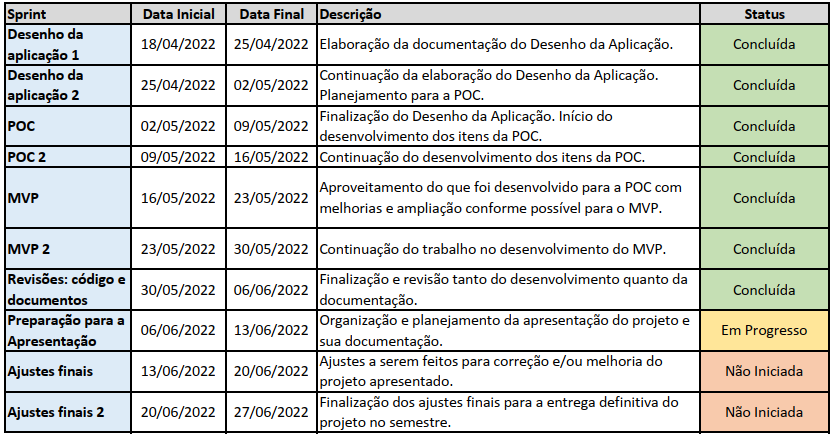
\includegraphics[width=0.8\textwidth]{../../imagens/cronograma-sprints.png}
		\fonte{Os Autores}
	\end{figure}
\end{frame}

%
%.........ORGANIZAÇÃO-DA-EQUIPE..........
%
\begin{frame}{Organização da Equipe} 
	\begin{figure}
		\centering
		\caption{\label{fig-org-team}Organização}
		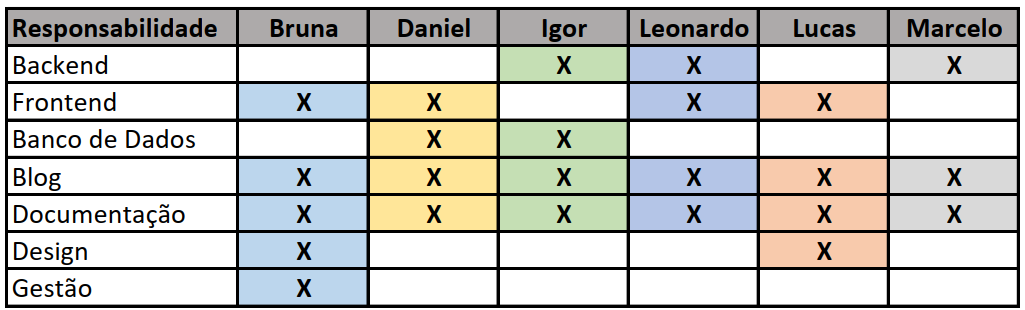
\includegraphics[width=\textwidth]{../../imagens/organizacao-equipe.png}
		\fonte{Os Autores}
	\end{figure}
\end{frame}

%
%.........>APLICAÇÃO<..........
%
\section{Aplicação}

%
%.........ARQUITETURA..........
%
\begin{frame}{Arquitetura} 
	\begin{figure}
		\centering
		\caption{\label{fig-arq-tec}Arquitetura de Aplicação}
		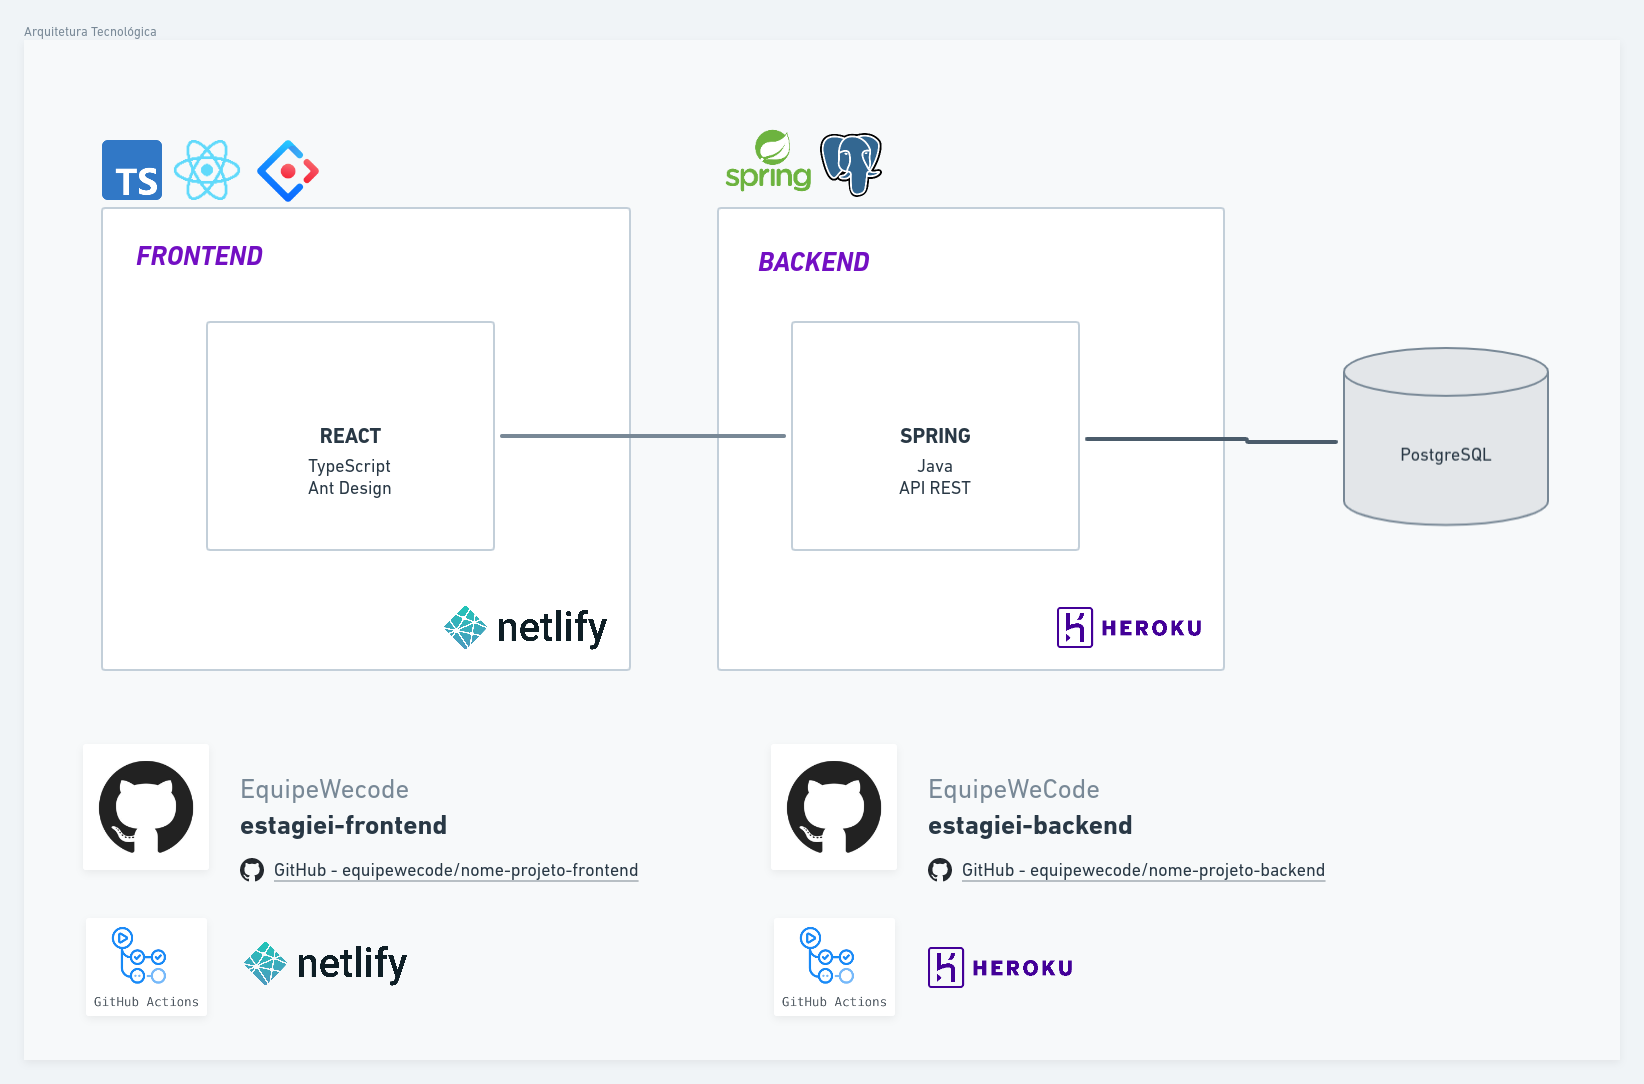
\includegraphics[width=0.8\textwidth]{../../imagens/arq-proj-arq-tec3.png}
		\fonte{Produzido pelos autores utilizando a ferramenta \textit{Whimsical}}
	\end{figure}
\end{frame}

%
%.........FRONT-END..........
%
\begin{frame}{Front-end}
	Telas:
	\begin{itemize}
		\item Login
		\item Listagem das vagas
		\item "Not found"
	\end{itemize}

	Internacionalização: Português (PT-BR) e Inglês (EN-US)
\end{frame}

%
%.........BACK-END..........
%
\begin{frame}{Back-end}
	Endpoints:
	\begin{itemize}
		\item api/loginEstudante
		\item api/estudante/{id}
		\item api/vaga
	\end{itemize}
	
\end{frame}

%
%.........ESCOPO-MVP..........
%
\begin{frame}{Implementações do MVP}
	\begin{itemize}
		\item Login com Google
		\item Lógica de Recomendação de Vagas para os estudantes
		\item Testes unitários
	\end{itemize}
\end{frame}

%
%.........DEMONSTRAÇÃO..........
%
\section{Demonstração}
\begin{frame}{Website} 
	%Add Logo
	\begin{figure}
		\centering
		
\includegraphics[width=\textwidth]{../../imagens/estagiei-logo.png}
		\fonte{Os Autores}
	\end{figure}
\end{frame}

\begin{comment}
\begin{frame}{Tabela}

% esse exemplo foi copiado diretamente do modelo de documento https://www.overleaf.com/project/58a3a66af9bb74023ba1bd56
\begin{table}
\centering
\caption{Um Exemplo de tabela}
\label{tab-exemplo}
\begin{tabular}{p{2.6cm}rrr}
    \hline
   \thead{Item} & \thead{Janeiro}  & \thead{Fevereiro}  & \thead{Março}  \\
    \hline
    Classes & 2  & 10 & 20  \\
    Linhas & 100  & 250 & 543 \\
    \hline
\end{tabular}
\fonte{Dados do Projeto}
\end{table}
\end{frame}

% Esse quadro veio do documento modelo onde são mostrados quadros errados e esse como a melhor forma de apresentar informações
\begin{frame}{Quadro}
\begin{quadro}
\centering
\tiny
\captionof{quadro}{Quadro de atividades de maneira mais clara e simples }
\label{quadro-poluido-limpo}
\begin{tabular}{|l|c|c|c|c|}
\hline
\thead{Responsável} & \thead{Atividade 1} & \thead{Atividade 2} & \thead{Atividade 3} & \thead{Atividade 4} \\
\hline
Pessoa 1 & \circlemark       &          &             & \circlemark         \\
\hline
Pessoa 2 & \circlemark       &          & \circlemark      &          \\
\hline
Pessoa 3 &          & \circlemark         &             &          \\
\hline
Pessoa 4 &          & \circlemark         & \circlemark      &         \\
\hline
\end{tabular}
\fonte{Os autores}
\end{quadro}

\end{frame}


\section{Quebras}

% foi utilizado enumerate para melhor visualização do exemplo, mas pode ser utilizado normalmente com itemize 
\begin{frame}[allowframebreaks=0.8]{Exemplo de quebra automatica}
    \begin{enumerate}
        \item aaaa
        \item aaaa
        \item aaaa
        \item aaaa
        \item aaaa
        \item aaaa
        \item aaaa
        \item aaaa
        \item aaaa
        \item aaaa
        \item aaaa
        \item aaaa
        \item aaaa
        \item aaaa
        \item aaaa
        \item aaaa
        \item aaaa
        \item aaaa
        \item aaaa
        \item aaaa
    \end{enumerate}
\end{frame}

\begin{frame}[allowframebreaks]{Exemplo de quebra manual}
    \begin{enumerate}
        \item aaaa
        \item aaaa
        \item aaaa
        \item aaaa
        \item aaaa
        \item aaaa
        \item aaaa
        \item aaaa
        \item aaaa
        \item aaaa
        \item aaaa
        
        \framebreak
        
        \item aaaa
        \item aaaa
        \item aaaa
        \item aaaa
        \item aaaa
        \item aaaa
        \item aaaa
        \item aaaa
        \item aaaa
    \end{enumerate}
\end{frame}




\section{Apresentando}
\begin{frame}{Dicas de Apresentação}
    \begin{itemize}
        
        \item Treine antes a apresentação, grave e assista para perceber os erros;
        
        \item Revise os slides e solicite que outras pessoas que não tenham participado da elaboração também façam essa revisão;
        
        \item Cronometre durante o treino para não exceder o tempo limite, durante a apresentação utilize também um cronometro para acompanhar o seu progresso, algumas ferramentas de apresentação auxiliam nesse procedimento
        
        \item A apresentação deve seguir o conteúdo do seu trabalho.
        
    \end{itemize}    
\end{frame}

%\author[Autor1 | \textit{Autor2}]{....}
\begin{frame}{Apresentações em Equipe}
    \begin{itemize}
        \item Coloque um marcador nos slides que permita facilmente lembrar quem é o responsável por aquela parte (alterar o autor do rodapé é uma solução simples e discreta, compare esse slide com o anterior);
        
        \item Todos devem conhecer a apresentação por completo de forma a ter uma contingencia caso um dos integrantes não possa apresentar;
        
        \item Cada participante deve ter um tempo razoável, não devem ter muita alternância durante a apresentação.
    \end{itemize}    
\end{frame}



% Seções somente para exemplificar as formatações possíveis para Agenda
\section{Alfa}

\section{Beta}

\section{Gama}


\section{Referências}

% Como nos documentos as referencias vão ser apresentadas de acordo com o uso do \cite... 
\begin{frame}[allowframebreaks]{Referências}
\bibliography{referencias.bib}
\end{frame}
\end{comment}
% * indica para não criar uma página de separação... e também não incluir na agenda
\section*{Dúvidas}

\newcommand{\urlApresentacao}{https://www.overleaf.com/read/hqmwmbvvskhr}
\begin{frame}{Dúvidas} 


% Endereço da Apresentação e contatos com QR-Code para facilitar acesso
% Se for uma apresentação remota é importante colocar no CHAT da ferramenta os dados para facilitar mais ainda

% dependendo do público não é necessário colocar os contatos
% Esse layout de duas colunas foi escolhido no caso para facilitar a captura dos qr codes já que a camera pode vir pela direita ou esquerda sem muita dificuldade


    \begin{columns}[t]
    
        \begin{column}{0.45\textwidth}
            \begin{block}{Dúvidas}
                \begin{itemize}
                  \item Perguntas ???
                \end{itemize}

                \begin{figure}
                    \centering
                    \qrcode{\urlApresentacao}
                    \caption*{Apresentação disponível em : \newline \url{\urlApresentacao}}
                \end{figure}

            \end{block}
        \end{column}
    
        % Exemplo de como gerar qr-code com email para contato....
        \begin{column}{0.55\textwidth}
            \begin{block}{Contatos}
                \begin{itemize}
                  \item Equipe WeCode
                  \item wecodetrabalho@gmail.com
                  \item \url{https://wecodeifsp.blogspot.com}
                \end{itemize}
    
                \begin{figure}
                    \centering
                    % utilizar a opção nolink caso queira deixar o qrcode preto sem o link
                    %\qrcode[nolink]{nome@aluno.ifsp.edu.br}
                    \qrcode{wecodetrabalho@gmail.com}
                \end{figure}
            \end{block}
        \end{column}
    \end{columns}




\end{frame}


\end{document}